\chapter{组合数学}

\index{组合数学}

\key{组合数学}研究计算对象组合的方法。
通常，目标是找到一种高效地计算组合的方式，
而不需要逐个生成每种组合。

作为一个例子，考虑如下问题：
计算将整数 $n$ 表示为正整数之和的方法数。
例如，$4$ 有 8 种表示方式：
\begin{multicols}{2}
\begin{itemize}
\item $1+1+1+1$
\item $1+1+2$
\item $1+2+1$
\item $2+1+1$
\item $2+2$
\item $3+1$
\item $1+3$
\item $4$
\end{itemize}
\end{multicols}

组合问题通常可以使用递归函数来解决。
在这个问题中，我们可以定义一个函数 $f(n)$，
它给出 $n$ 的表示方法数。
例如，根据上例，$f(4)=8$。
该函数的值可以按如下方式递归计算：
\begin{equation*}
    f(n) = \begin{cases}
               1               & n = 0\\
               f(0)+f(1)+\cdots+f(n-1) & n > 0\\
           \end{cases}
\end{equation*}
基本情形是 $f(0)=1$，
因为空和表示数字 0。
然后，如果 $n>0$，我们考虑选择和的第一个数的所有方式。
如果第一个数是 $k$，
则和的剩余部分有 $f(n-k)$ 种表示方式。
因此，我们计算所有形如 $f(n-k)$（其中 $k<n$）的值之和。

该函数的前几个值为：
\[
\begin{array}{lcl}
f(0) & = & 1 \\
f(1) & = & 1 \\
f(2) & = & 2 \\
f(3) & = & 4 \\
f(4) & = & 8 \\
\end{array}
\]

有时，递归公式可以用一个闭式公式代替。
在这个问题中，
\[
f(n)=2^{n-1},
\]
这基于如下事实：和式中加号有 $n-1$ 个可能的位置，
我们可以选择其中的任意子集。

\section{二项式系数}

\index{二项式系数}

\key{二项式系数} ${n \choose k}$
等于从 $n$ 个元素的集合中选取 $k$ 个元素的子集的方法数。
例如，${5 \choose 3}=10$，
因为集合 $\{1,2,3,4,5\}$
有 10 个含 3 个元素的子集：
\[ \{1,2,3\}, \{1,2,4\}, \{1,2,5\}, \{1,3,4\}, \{1,3,5\}, 
\{1,4,5\}, \{2,3,4\}, \{2,3,5\}, \{2,4,5\}, \{3,4,5\} \]

\subsubsection{公式1}

二项式系数可以按如下方式递归计算：

\[
{n \choose k}  =  {n-1 \choose k-1} + {n-1 \choose k}
\]

其想法是固定集合中的一个元素 $x$。
如果 $x$ 包含在子集中，
我们需要从 $n-1$ 个元素中选择 $k-1$ 个元素；
如果 $x$ 不包含在子集中，
我们需要从 $n-1$ 个元素中选择 $k$ 个元素。

递归的基本情形是
\[
{n \choose 0}  =  {n \choose n} = 1,
\]
因为构造一个空子集和包含所有元素的子集
总是恰好有一种方法。

\subsubsection{公式2}

计算二项式系数的另一种方法如下：
\[
{n \choose k}  =  \frac{n!}{k!(n-k)!}.
\]

$n$ 个元素有 $n!$ 种排列。
我们遍历所有排列，并总是将排列的前 $k$ 个元素
包含在子集中。
由于子集内部和子集外部元素的顺序都不重要，
所以结果需要除以 $k!$ 和 $(n-k)!$。

\subsubsection{性质}

对于二项式系数，
\[
{n \choose k}  =  {n \choose n-k},
\]
因为我们实际上将 $n$ 个元素的集合划分为
两个子集：第一个包含 $k$ 个元素，
第二个包含 $n-k$ 个元素。

二项式系数之和为
\[
{n \choose 0}+{n \choose 1}+{n \choose 2}+\ldots+{n \choose n}=2^n.
\]

“二项式系数”这个名称的由来可以从
二项式 $(a+b)$ 的 $n$ 次幂中看出：

\[ (a+b)^n =
{n \choose 0} a^n b^0 + 
{n \choose 1} a^{n-1} b^1 +
\ldots + 
{n \choose n-1} a^1 b^{n-1} +
{n \choose n} a^0 b^n. \]

\index{杨辉三角}

二项式系数也出现在\key{杨辉三角}中，
其中每个值等于其上方两个值之和：
\begin{center}
\begin{tikzpicture}{0.9}
\node at (0,0) {1};
\node at (-0.5,-0.5) {1};
\node at (0.5,-0.5) {1};
\node at (-1,-1) {1};
\node at (0,-1) {2};
\node at (1,-1) {1};
\node at (-1.5,-1.5) {1};
\node at (-0.5,-1.5) {3};
\node at (0.5,-1.5) {3};
\node at (1.5,-1.5) {1};
\node at (-2,-2) {1};
\node at (-1,-2) {4};
\node at (0,-2) {6};
\node at (1,-2) {4};
\node at (2,-2) {1};
\node at (-2,-2.5) {$\ldots$};
\node at (-1,-2.5) {$\ldots$};
\node at (0,-2.5) {$\ldots$};
\node at (1,-2.5) {$\ldots$};
\node at (2,-2.5) {$\ldots$};
\end{tikzpicture}
\end{center}

\subsubsection{盒与球}

“盒与球”是一个有用的模型，
其中我们计算将 $k$ 个球放入 $n$ 个盒子的方法数。
让我们考虑三种场景：

\textit{场景1}：每个盒子最多包含
一个球。
例如，当 $n=5$ 且 $k=2$ 时，
有 10 种方案：

\begin{center}
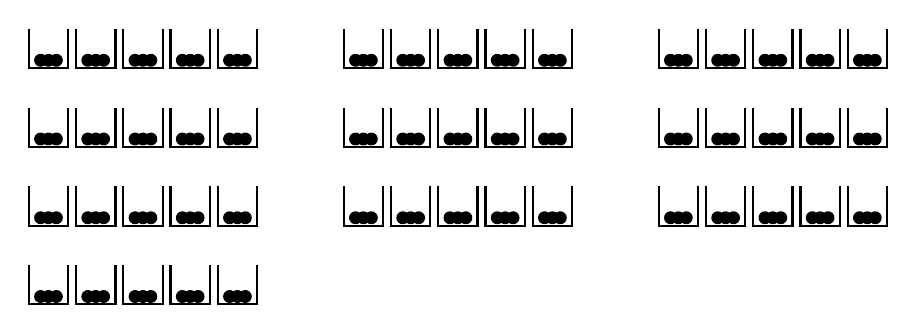
\begin{tikzpicture}[scale=0.5]
\newcommand\lax[3]{
\path[draw,thick,-] (#1-0.5,#2+0.5) -- (#1-0.5,#2-0.5) --
                    (#1+0.5,#2-0.5) -- (#1+0.5,#2+0.5);
\ifthenelse{\equal{#3}{1}}{\draw[fill=black] (#1,#2-0.3) circle (0.15);}{}
\ifthenelse{\equal{#3}{2}}{\draw[fill=black] (#1-0.2,#2-0.3) circle (0.15);}{}
\ifthenelse{\equal{#3}{2}}{\draw[fill=black] (#1+0.2,#2-0.3) circle (0.15);}{}
}
\newcommand\laa[7]{
    \lax{#1}{#2}{#3}
    \lax{#1+1.2}{#2}{#4}
    \lax{#1+2.4}{#2}{#5}
    \lax{#1+3.6}{#2}{#6}
    \lax{#1+4.8}{#2}{#7}
}

\laa{0}{0}{1}{1}{0}{0}{0}
\laa{0}{-2}{1}{0}{1}{0}{0}
\laa{0}{-4}{1}{0}{0}{1}{0}
\laa{0}{-6}{1}{0}{0}{0}{1}
\laa{8}{0}{0}{1}{1}{0}{0}
\laa{8}{-2}{0}{1}{0}{1}{0}
\laa{8}{-4}{0}{1}{0}{0}{1}
\laa{16}{0}{0}{0}{1}{1}{0}
\laa{16}{-2}{0}{0}{1}{0}{1}
\laa{16}{-4}{0}{0}{0}{1}{1}

\end{tikzpicture}
\end{center}

在这个场景中，答案直接就是
二项式系数 ${n \choose k}$。

\textit{场景2}：一个盒子可以包含多个球。
例如，当 $n=5$ 且 $k=2$ 时，
有 15 种方案：

\begin{center}
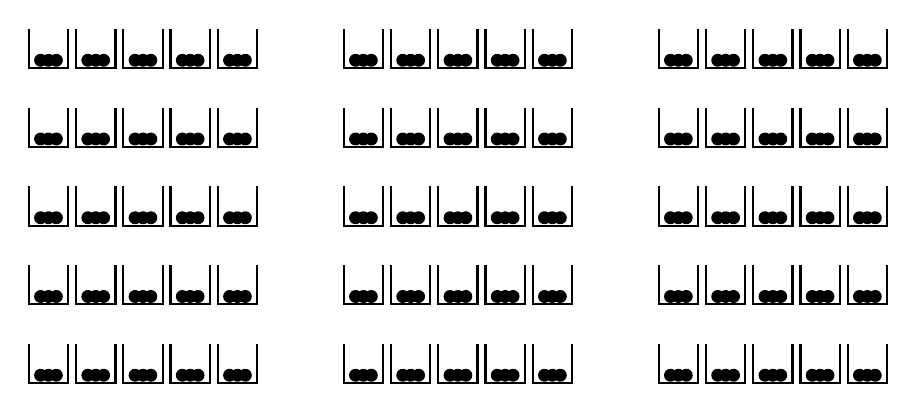
\begin{tikzpicture}[scale=0.5]
\newcommand\lax[3]{
\path[draw,thick,-] (#1-0.5,#2+0.5) -- (#1-0.5,#2-0.5) --
                    (#1+0.5,#2-0.5) -- (#1+0.5,#2+0.5);
\ifthenelse{\equal{#3}{1}}{\draw[fill=black] (#1,#2-0.3) circle (0.15);}{}
\ifthenelse{\equal{#3}{2}}{\draw[fill=black] (#1-0.2,#2-0.3) circle (0.15);}{}
\ifthenelse{\equal{#3}{2}}{\draw[fill=black] (#1+0.2,#2-0.3) circle (0.15);}{}
}
\newcommand\laa[7]{
    \lax{#1}{#2}{#3}
    \lax{#1+1.2}{#2}{#4}
    \lax{#1+2.4}{#2}{#5}
    \lax{#1+3.6}{#2}{#6}
    \lax{#1+4.8}{#2}{#7}
}

\laa{0}{0}{2}{0}{0}{0}{0}
\laa{0}{-2}{1}{1}{0}{0}{0}
\laa{0}{-4}{1}{0}{1}{0}{0}
\laa{0}{-6}{1}{0}{0}{1}{0}
\laa{0}{-8}{1}{0}{0}{0}{1}
\laa{8}{0}{0}{2}{0}{0}{0}
\laa{8}{-2}{0}{1}{1}{0}{0}
\laa{8}{-4}{0}{1}{0}{1}{0}
\laa{8}{-6}{0}{1}{0}{0}{1}
\laa{8}{-8}{0}{0}{2}{0}{0}
\laa{16}{0}{0}{0}{1}{1}{0}
\laa{16}{-2}{0}{0}{1}{0}{1}
\laa{16}{-4}{0}{0}{0}{2}{0}
\laa{16}{-6}{0}{0}{0}{1}{1}
\laa{16}{-8}{0}{0}{0}{0}{2}

\end{tikzpicture}
\end{center}

将球放入盒子的过程可以表示为一个字符串，
由符号“o”和“$\rightarrow$”组成。
初始时，假设我们站在最左边的盒子处。
符号“o”表示我们在当前盒子中放入一个球，
符号“$\rightarrow$”表示我们向右移动到
下一个盒子。

使用这种表示法，每个方案是一个包含 $k$ 个符号“o”和
$n-1$ 个符号“$\rightarrow$”的字符串。
例如，上图中右上角的方案对应字符串
“$\rightarrow$ $\rightarrow$ o $\rightarrow$ o $\rightarrow$”。
因此，方案数为
${k+n-1 \choose k}$。

\textit{场景3}：每个盒子最多包含一个球，
此外，没有两个相邻的盒子可以同时包含球。
例如，当 $n=5$ 且 $k=2$ 时，
有 6 种方案：


\begin{center}
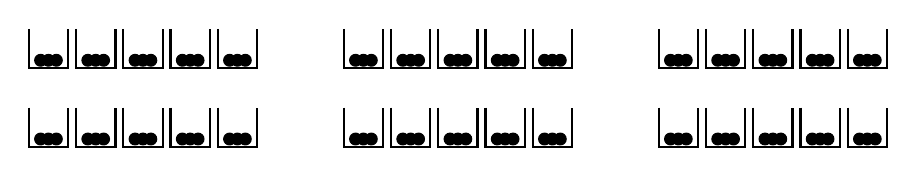
\begin{tikzpicture}[scale=0.5]
\newcommand\lax[3]{
\path[draw,thick,-] (#1-0.5,#2+0.5) -- (#1-0.5,#2-0.5) --
                    (#1+0.5,#2-0.5) -- (#1+0.5,#2+0.5);
\ifthenelse{\equal{#3}{1}}{\draw[fill=black] (#1,#2-0.3) circle (0.15);}{}
\ifthenelse{\equal{#3}{2}}{\draw[fill=black] (#1-0.2,#2-0.3) circle (0.15);}{}
\ifthenelse{\equal{#3}{2}}{\draw[fill=black] (#1+0.2,#2-0.3) circle (0.15);}{}
}
\newcommand\laa[7]{
    \lax{#1}{#2}{#3}
    \lax{#1+1.2}{#2}{#4}
    \lax{#1+2.4}{#2}{#5}
    \lax{#1+3.6}{#2}{#6}
    \lax{#1+4.8}{#2}{#7}
}

\laa{0}{0}{1}{0}{1}{0}{0}
\laa{0}{-2}{1}{0}{0}{1}{0}
\laa{8}{0}{1}{0}{0}{0}{1}
\laa{8}{-2}{0}{1}{0}{1}{0}
\laa{16}{0}{0}{1}{0}{0}{1}
\laa{16}{-2}{0}{0}{1}{0}{1}
\end{tikzpicture}
\end{center}

在这个场景中，我们可以假设 $k$ 个球初始已放入盒子中，
并且每两个相邻的球之间有一个空盒子。
剩余的任务是选择剩余空盒子的位置。
这样的盒子有 $n-2k+1$ 个，
它们的位置有 $k+1$ 个可选位置。
因此，使用场景2的公式，
方案数为
${n-k+1 \choose n-2k+1}$。

\subsubsection{多项式系数}

\index{多项式系数}

\key{多项式系数}
\[ {n \choose k_1,k_2,\ldots,k_m} = \frac{n!}{k_1! k_2! \cdots k_m!}, \]
等于将 $n$ 个元素划分为
大小为 $k_1,k_2,\ldots,k_m$ 的子集的方法数，
其中 $k_1+k_2+\cdots+k_m=n$。
多项式系数可以看作是二项式系数的推广；
如果 $m=2$，上述公式对应于二项式系数公式。

\section{卡特兰数}

\index{卡特兰数}

\key{卡特兰数}
%\footnote{E. C. Catalan (1814--1894) 是一位比利时数学家。}
$C_n$ 等于由
$n$ 个左括号和 $n$ 个右括号组成的
合法括号表达式的个数。

例如，$C_3=5$，因为
我们可以用三个左括号和三个右括号
构造以下括号表达式：

\begin{itemize}[noitemsep]
\item \texttt{()()()}
\item \texttt{(())()}
\item \texttt{()(())}
\item \texttt{((()))}
\item \texttt{(()())}
\end{itemize}

\subsubsection{括号表达式}

\index{括号表达式}

什么是\emph{合法的括号表达式}？
以下规则精确地定义了所有
合法的括号表达式：

\begin{itemize}
\item 空的括号表达式是合法的。
\item 如果表达式 $A$ 是合法的，
那么表达式
\texttt{(}$A$\texttt{)} 也是合法的。
\item 如果表达式 $A$ 和 $B$ 都是合法的，
那么表达式 $AB$ 也是合法的。
\end{itemize}

另一种描述合法括号表达式的方式是：
如果我们选择这样一个表达式的任意前缀，
它包含的左括号数量必须至少
不少于右括号数量。
此外，完整的表达式必须
包含相等数量的左括号和右括号。

\subsubsection{公式1}

卡特兰数可以使用以下公式计算
\[ C_n = \sum_{i=0}^{n-1} C_{i} C_{n-i-1}.\]

该求和遍历将表达式划分为两部分的所有方式，
使得两部分都是合法表达式，
且第一部分尽可能短但不为空。
对于任意 $i$，第一部分包含 $i+1$ 对括号，
表达式数量是以下值的乘积：

\begin{itemize}
\item $C_{i}$：使用第一部分的括号构造表达式的方法数，
不计算最外层的括号
\item $C_{n-i-1}$：使用第二部分的括号构造表达式的方法数
\end{itemize}

基本情形是 $C_0=1$，
因为我们可以用零对括号构造一个空括号表达式。

\subsubsection{公式2}

卡特兰数也可以使用二项式系数计算：
\[ C_n = \frac{1}{n+1} {2n \choose n}\]
该公式可以解释如下：

总共有 ${2n \choose n}$ 种方法构造一个
（不一定合法的）包含 $n$ 个左括号
和 $n$ 个右括号的括号表达式。
让我们计算其中\emph{不}合法的
表达式数量。

如果一个括号表达式不合法，
它必须包含一个前缀，其中右括号的数量
超过左括号的数量。
其想法是将属于这样一个前缀的每个括号反转。
例如，表达式
\texttt{())()(} 包含前缀 \texttt{())}，
反转前缀后，表达式变为 \texttt{)((()(}。

所得表达式由 $n+1$ 个左括号和 $n-1$ 个右括号组成。
这样的表达式数量为 ${2n \choose n+1}$，
等于不合法的括号表达式数量。
因此，合法的括号表达式数量
可以使用以下公式计算
\[{2n \choose n}-{2n \choose n+1} = {2n \choose n} - \frac{n}{n+1} {2n \choose n} = \frac{1}{n+1} {2n \choose n}.\]

\subsubsection{树的计数}

卡特兰数也与树有关：

\begin{itemize}
\item $n$ 个结点的二叉树有 $C_n$ 棵
\item $n$ 个结点的有根树有 $C_{n-1}$ 棵
\end{itemize}
\noindent
例如，对于 $C_3=5$，二叉树为

\begin{center}
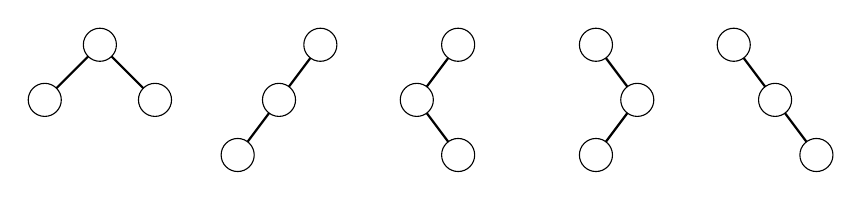
\begin{tikzpicture}[scale=0.7]
\path[draw,thick,-] (0,0) -- (-1,-1);
\path[draw,thick,-] (0,0) -- (1,-1);
\draw[fill=white] (0,0) circle (0.3);
\draw[fill=white] (-1,-1) circle (0.3);
\draw[fill=white] (1,-1) circle (0.3);

\path[draw,thick,-] (4,0) -- (4-0.75,-1) -- (4-1.5,-2);
\draw[fill=white] (4,0) circle (0.3);
\draw[fill=white] (4-0.75,-1) circle (0.3);
\draw[fill=white] (4-1.5,-2) circle (0.3);

\path[draw,thick,-] (6.5,0) -- (6.5-0.75,-1) -- (6.5-0,-2);
\draw[fill=white] (6.5,0) circle (0.3);
\draw[fill=white] (6.5-0.75,-1) circle (0.3);
\draw[fill=white] (6.5-0,-2) circle (0.3);

\path[draw,thick,-] (9,0) -- (9+0.75,-1) -- (9-0,-2);
\draw[fill=white] (9,0) circle (0.3);
\draw[fill=white] (9+0.75,-1) circle (0.3);
\draw[fill=white] (9-0,-2) circle (0.3);

\path[draw,thick,-] (11.5,0) -- (11.5+0.75,-1) -- (11.5+1.5,-2);
\draw[fill=white] (11.5,0) circle (0.3);
\draw[fill=white] (11.5+0.75,-1) circle (0.3);
\draw[fill=white] (11.5+1.5,-2) circle (0.3);
\end{tikzpicture}
\end{center}
其中有根树为
\begin{center}
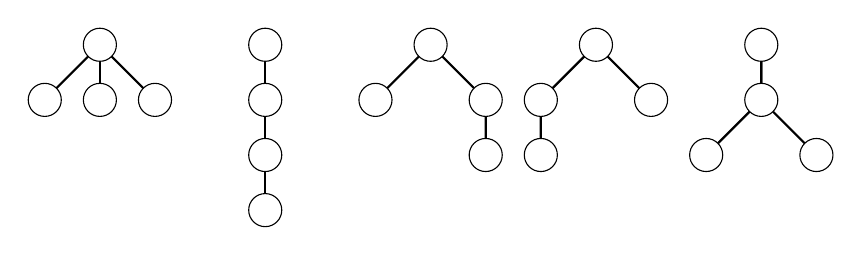
\begin{tikzpicture}[scale=0.7]
\path[draw,thick,-] (0,0) -- (-1,-1);
\path[draw,thick,-] (0,0) -- (0,-1);
\path[draw,thick,-] (0,0) -- (1,-1);
\draw[fill=white] (0,0) circle (0.3);
\draw[fill=white] (-1,-1) circle (0.3);
\draw[fill=white] (0,-1) circle (0.3);
\draw[fill=white] (1,-1) circle (0.3);

\path[draw,thick,-] (3,0) -- (3,-1) -- (3,-2) -- (3,-3);
\draw[fill=white] (3,0) circle (0.3);
\draw[fill=white] (3,-1) circle (0.3);
\draw[fill=white] (3,-2) circle (0.3);
\draw[fill=white] (3,-3) circle (0.3);

\path[draw,thick,-] (6+0,0) -- (6-1,-1);
\path[draw,thick,-] (6+0,0) -- (6+1,-1) -- (6+1,-2);
\draw[fill=white] (6+0,0) circle (0.3);
\draw[fill=white] (6-1,-1) circle (0.3);
\draw[fill=white] (6+1,-1) circle (0.3);
\draw[fill=white] (6+1,-2) circle (0.3);

\path[draw,thick,-] (9+0,0) -- (9+1,-1);
\path[draw,thick,-] (9+0,0) -- (9-1,-1) -- (9-1,-2);
\draw[fill=white] (9+0,0) circle (0.3);
\draw[fill=white] (9+1,-1) circle (0.3);
\draw[fill=white] (9-1,-1) circle (0.3);
\draw[fill=white] (9-1,-2) circle (0.3);

\path[draw,thick,-] (12+0,0) -- (12+0,-1) -- (12-1,-2);
\path[draw,thick,-] (12+0,0) -- (12+0,-1) -- (12+1,-2);
\draw[fill=white] (12+0,0) circle (0.3);
\draw[fill=white] (12+0,-1) circle (0.3);
\draw[fill=white] (12-1,-2) circle (0.3);
\draw[fill=white] (12+1,-2) circle (0.3);

\end{tikzpicture}
\end{center}

\section{容斥原理}

\index{容斥原理}

\key{容斥原理}是一种技巧，
可用于计算集合并集的大小，
当交集的大小已知时，反之亦然。
该技巧的一个简单例子是公式
\[ |A \cup B| = |A| + |B| - |A \cap B|,\]
其中 $A$ 和 $B$ 是集合，$|X|$
表示 $X$ 的大小。
该公式可以如下说明：

\begin{center}
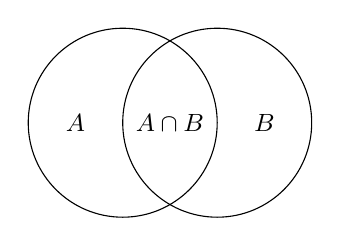
\begin{tikzpicture}[scale=0.8]

\draw (0,0) circle (1.5);
\draw (1.5,0) circle (1.5);

\node at (-0.75,0) {\small $A$};
\node at (2.25,0) {\small $B$};
\node at (0.75,0) {\small $A \cap B$};

\end{tikzpicture}
\end{center}

我们的目标是计算并集 $A \cup B$ 的大小，
它对应于至少属于一个圆的区域面积。
图中显示，我们可以通过先将 $A$ 和 $B$ 的面积
相加，然后减去 $A \cap B$ 的面积来计算 $A \cup B$ 的面积。

同样的思想可以应用于更多集合的情况。
当有三个集合时，容斥公式为
\[ |A \cup B \cup C| = |A| + |B| + |C| - |A \cap B|  - |A \cap C|  - |B \cap C| + |A \cap B \cap C| \]
对应的图为

\begin{center}
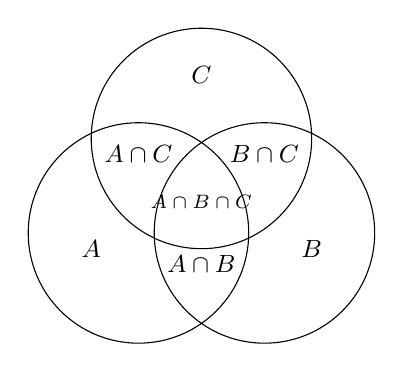
\begin{tikzpicture}[scale=0.8]

\draw (0,0) circle (1.75);
\draw (2,0) circle (1.75);
\draw (1,1.5) circle (1.75);

\node at (-0.75,-0.25) {\small $A$};
\node at (2.75,-0.25) {\small $B$};
\node at (1,2.5) {\small $C$};
\node at (1,-0.5) {\small $A \cap B$};
\node at (0,1.25) {\small $A \cap C$};
\node at (2,1.25) {\small $B \cap C$};
\node at (1,0.5) {\scriptsize $A \cap B \cap C$};

\end{tikzpicture}
\end{center}

在一般情况下，并集
$X_1 \cup X_2 \cup \cdots \cup X_n$
的大小可以通过遍历所有可能的
包含集合 $X_1,X_2,\ldots,X_n$ 中某些集合的交集来计算。
如果交集包含奇数个集合，
其大小被加到答案中，
否则其大小被从答案中减去。

注意，也有类似的公式
可以从并集的大小计算交集的大小。例如，
\[ |A \cap B| = |A| + |B| - |A \cup B|\]
和
\[ |A \cap B \cap C| = |A| + |B| + |C| - |A \cup B|  - |A \cup C|  - |B \cup C| + |A \cup B \cup C| .\]

\subsubsection{错排}

\index{错排}

作为例子，让我们计算元素 $\{1,2,\ldots,n\}$ 的\key{错排}数量，
即没有元素留在原位的排列。
例如，当 $n=3$ 时，有两个错排：
$(2,3,1)$ 和 $(3,1,2)$。

解决这个问题的一种方法是使用容斥原理。
令 $X_k$ 为在位置 $k$ 处包含元素 $k$ 的排列集合。
例如，当 $n=3$ 时，集合如下：
\[
\begin{array}{lcl}
X_1 & = & \{(1,2,3),(1,3,2)\} \\
X_2 & = & \{(1,2,3),(3,2,1)\} \\
X_3 & = & \{(1,2,3),(2,1,3)\} \\
\end{array}
\]
使用这些集合，错排数量等于
\[ n! - |X_1 \cup X_2 \cup \cdots \cup X_n|, \]
因此只需计算并集的大小。
使用容斥原理，这归结为
计算交集的大小，这可以高效完成。
例如，当 $n=3$ 时，$|X_1 \cup X_2 \cup X_3|$ 的大小为
\[
\begin{array}{lcl}
 & & |X_1| + |X_2| + |X_3| - |X_1 \cap X_2|  - |X_1 \cap X_3|  - |X_2 \cap X_3| + |X_1 \cap X_2 \cap X_3| \\
 & = & 2+2+2-1-1-1+1 \\
 & = & 4, \\
\end{array}
\]
所以方案数为 $3!-4=2$。

事实上，这个问题也可以不使用容斥原理解决。
令 $f(n)$ 表示 $\{1,2,\ldots,n\}$ 的错排数。
我们可以使用以下递归公式：

\begin{equation*}
    f(n) = \begin{cases}
               0               & n = 1\\
               1               & n = 2\\
               (n-1)(f(n-2) + f(n-1)) & n>2 \\
           \end{cases}
\end{equation*}

该公式可以通过考虑元素 1 在错排中
如何变化的可能性来推导。
有 $n-1$ 种方法选择一个元素 $x$ 来替换元素 1。
对于每种选择，有两个选项：

\textit{选项1：}我们也用元素 1 替换元素 $x$。
之后，剩余的任务是构造 $n-2$ 个元素的错排。

\textit{选项2：}我们用 1 以外的某个元素替换元素 $x$。
现在我们需要构造 $n-1$ 个元素的错排，
因为我们不能用元素 1 替换元素 $x$，
而所有其他元素都必须改变。

\section{Burnside引理}

\index{Burnside引理}

\key{Burnside引理}
%\footnote{事实上，Burnside并没有发现这个引理；他只是在其著作 \cite{bur97} 中提到了它。}
可用于计算组合数量，
使得每组对称组合只计算一个代表。
Burnside引理指出，组合数量为
\[\sum_{k=1}^n \frac{c(k)}{n},\]
其中有 $n$ 种改变组合位置的方式，
$c(k)$ 是当应用第 $k$ 种方式时
保持不变的组合数。

作为例子，让我们计算由 $n$ 颗珠子组成的项链数量，
其中每颗珠子有 $m$ 种可能的颜色。
如果两条项链在旋转后相似，则它们是对称的。
例如，项链
\begin{center}
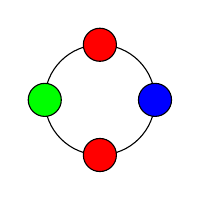
\begin{tikzpicture}[scale=0.7]
\draw[fill=white] (0,0) circle (1);
\draw[fill=red] (0,1) circle (0.3);
\draw[fill=blue] (1,0) circle (0.3);
\draw[fill=red] (0,-1) circle (0.3);
\draw[fill=green] (-1,0) circle (0.3);
\end{tikzpicture}
\end{center}
有以下对称项链：
\begin{center}
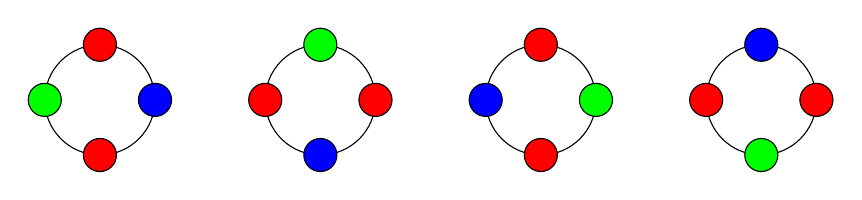
\begin{tikzpicture}[scale=0.7]
\draw[fill=white] (0,0) circle (1);
\draw[fill=red] (0,1) circle (0.3);
\draw[fill=blue] (1,0) circle (0.3);
\draw[fill=red] (0,-1) circle (0.3);
\draw[fill=green] (-1,0) circle (0.3);

\draw[fill=white] (4,0) circle (1);
\draw[fill=green] (4+0,1) circle (0.3);
\draw[fill=red] (4+1,0) circle (0.3);
\draw[fill=blue] (4+0,-1) circle (0.3);
\draw[fill=red] (4+-1,0) circle (0.3);

\draw[fill=white] (8,0) circle (1);
\draw[fill=red] (8+0,1) circle (0.3);
\draw[fill=green] (8+1,0) circle (0.3);
\draw[fill=red] (8+0,-1) circle (0.3);
\draw[fill=blue] (8+-1,0) circle (0.3);

\draw[fill=white] (12,0) circle (1);
\draw[fill=blue] (12+0,1) circle (0.3);
\draw[fill=red] (12+1,0) circle (0.3);
\draw[fill=green] (12+0,-1) circle (0.3);
\draw[fill=red] (12+-1,0) circle (0.3);
\end{tikzpicture}
\end{center}
有 $n$ 种方式改变项链的位置，
因为我们可以将其顺时针旋转
$0,1,\ldots,n-1$ 步。
如果步数为 0，
所有 $m^n$ 条项链保持不变；
如果步数为 1，
只有每颗珠子颜色相同的 $m$ 条项链保持不变。

更一般地，当步数为 $k$ 时，共有
\[m^{\textrm{gcd}(k,n)}\]
条项链保持不变，
其中 $\textrm{gcd}(k,n)$ 是 $k$ 和 $n$ 的最大公约数。
其原因是大小为 $\textrm{gcd}(k,n)$ 的珠子块
将互相替换。
因此，根据Burnside引理，
项链数量为
\[\sum_{i=0}^{n-1} \frac{m^{\textrm{gcd}(i,n)}}{n}. \]
例如，长度为 4、使用 3 种颜色的项链数量为
\[\frac{3^4+3+3^2+3}{4} = 24. \]

\section{Cayley公式}

\index{Cayley公式}

\key{Cayley公式}
% \footnote{虽然该公式以 A. Cayley 命名，
% 他在1889年研究了它，但更早由 C. W. Borchardt 于1860年发现。}
指出，包含 $n$ 个结点的有标号树
共有 $n^{n-2}$ 棵。
结点标记为 $1,2,\ldots,n$，
两棵树如果结构或标记不同，
则它们是不同的。

\begin{samepage}
例如，当 $n=4$ 时，有标号树的数量为 $4^{4-2}=16$：

\begin{center}
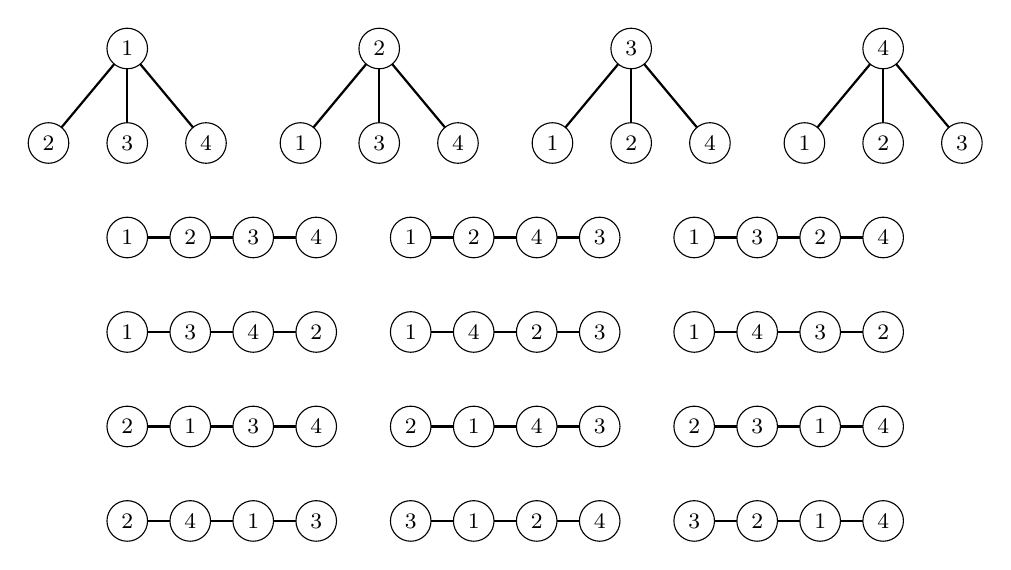
\begin{tikzpicture}[scale=0.8]
\footnotesize

\newcommand\puua[6]{
\path[draw,thick,-] (#1,#2) -- (#1-1.25,#2-1.5);
\path[draw,thick,-] (#1,#2) -- (#1,#2-1.5);
\path[draw,thick,-] (#1,#2) -- (#1+1.25,#2-1.5);
\node[draw, circle, fill=white] at (#1,#2) {#3};
\node[draw, circle, fill=white] at (#1-1.25,#2-1.5) {#4};
\node[draw, circle, fill=white] at (#1,#2-1.5) {#5};
\node[draw, circle, fill=white] at (#1+1.25,#2-1.5) {#6};
}
\newcommand\puub[6]{
\path[draw,thick,-] (#1,#2) -- (#1+1,#2);
\path[draw,thick,-] (#1+1,#2) -- (#1+2,#2);
\path[draw,thick,-] (#1+2,#2) -- (#1+3,#2);
\node[draw, circle, fill=white] at (#1,#2) {#3};
\node[draw, circle, fill=white] at (#1+1,#2) {#4};
\node[draw, circle, fill=white] at (#1+2,#2) {#5};
\node[draw, circle, fill=white] at (#1+3,#2) {#6};
}

\puua{0}{0}{1}{2}{3}{4}
\puua{4}{0}{2}{1}{3}{4}
\puua{8}{0}{3}{1}{2}{4}
\puua{12}{0}{4}{1}{2}{3}

\puub{0}{-3}{1}{2}{3}{4}
\puub{4.5}{-3}{1}{2}{4}{3}
\puub{9}{-3}{1}{3}{2}{4}
\puub{0}{-4.5}{1}{3}{4}{2}
\puub{4.5}{-4.5}{1}{4}{2}{3}
\puub{9}{-4.5}{1}{4}{3}{2}
\puub{0}{-6}{2}{1}{3}{4}
\puub{4.5}{-6}{2}{1}{4}{3}
\puub{9}{-6}{2}{3}{1}{4}
\puub{0}{-7.5}{2}{4}{1}{3}
\puub{4.5}{-7.5}{3}{1}{2}{4}
\puub{9}{-7.5}{3}{2}{1}{4}
\end{tikzpicture}
\end{center}
\end{samepage}

接下来我们将看到如何使用Prüfer编码
来推导Cayley公式。

\subsubsection{Prüfer编码}

\index{Prüfer编码}

\key{Prüfer编码}
%\footnote{1918年，H. Prüfer 使用 Prüfer 编码证明了 Cayley 定理 \cite{pru18}。}
是一个描述有标号树的
$n-2$ 个数的序列。
该编码的构造过程是从树中移除 $n-2$ 个叶子。
在每一步中，移除标记最小的叶子，
并将其唯一邻居的标记添加到编码中。

例如，让我们计算以下图的Prüfer编码：
\begin{center}
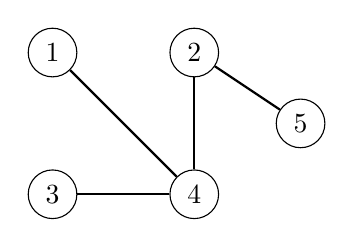
\begin{tikzpicture}[scale=0.9]
\node[draw, circle] (1) at (2,3) {$1$};
\node[draw, circle] (2) at (4,3) {$2$};
\node[draw, circle] (3) at (2,1) {$3$};
\node[draw, circle] (4) at (4,1) {$4$};
\node[draw, circle] (5) at (5.5,2) {$5$};

\path[draw,thick,-] (1) -- (4);
\path[draw,thick,-] (3) -- (4);
\path[draw,thick,-] (2) -- (4);
\path[draw,thick,-] (2) -- (5);
\end{tikzpicture}
\end{center}

首先我们移除结点 1，并将结点 4 添加到编码中：
\begin{center}
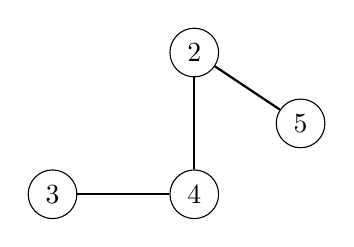
\begin{tikzpicture}[scale=0.9]
%\node[draw, circle] (1) at (2,3) {$1$};
\node[draw, circle] (2) at (4,3) {$2$};
\node[draw, circle] (3) at (2,1) {$3$};
\node[draw, circle] (4) at (4,1) {$4$};
\node[draw, circle] (5) at (5.5,2) {$5$};

%\path[draw,thick,-] (1) -- (4);
\path[draw,thick,-] (3) -- (4);
\path[draw,thick,-] (2) -- (4);
\path[draw,thick,-] (2) -- (5);
\end{tikzpicture}
\end{center}

然后我们移除结点 3，并将结点 4 添加到编码中：
\begin{center}
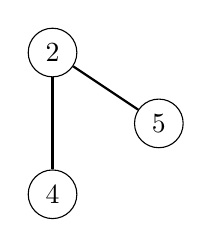
\begin{tikzpicture}[scale=0.9]
%\node[draw, circle] (1) at (2,3) {$1$};
\node[draw, circle] (2) at (4,3) {$2$};
%\node[draw, circle] (3) at (2,1) {$3$};
\node[draw, circle] (4) at (4,1) {$4$};
\node[draw, circle] (5) at (5.5,2) {$5$};

%\path[draw,thick,-] (1) -- (4);
%\path[draw,thick,-] (3) -- (4);
\path[draw,thick,-] (2) -- (4);
\path[draw,thick,-] (2) -- (5);
\end{tikzpicture}
\end{center}

最后我们移除结点 4，并将结点 2 添加到编码中：
\begin{center}
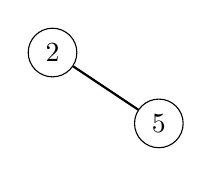
\begin{tikzpicture}[scale=0.9]
%\node[draw, circle] (1) at (2,3) {$1$};
\node[draw, circle] (2) at (4,3) {$2$};
%\node[draw, circle] (3) at (2,1) {$3$};
%\node[draw, circle] (4) at (4,1) {$4$};
\node[draw, circle] (5) at (5.5,2) {$5$};

%\path[draw,thick,-] (1) -- (4);
%\path[draw,thick,-] (3) -- (4);
%\path[draw,thick,-] (2) -- (4);
\path[draw,thick,-] (2) -- (5);
\end{tikzpicture}
\end{center}

因此，该图的Prüfer编码为 $[4,4,2]$。

我们可以为任何树构造Prüfer编码，
更重要的是，
可以从Prüfer编码重构原始树。
因此，$n$ 个结点的有标号树数量等于
$n^{n-2}$，即大小为 $n$ 的Prüfer编码数量。
